\documentclass[a4paper]{article}

\usepackage{INTERSPEECH2015}

\usepackage{graphicx}
\usepackage{hyperref}
\usepackage{array}
\usepackage{float}
\usepackage{amssymb,amsmath,bm}
\usepackage{textcomp}
\usepackage[T1]{fontenc}
\usepackage[utf8]{inputenc}
\graphicspath{ {png/} }

\def\vec#1{\ensuremath{\bm{{#1}}}}
\def\mat#1{\vec{#1}}
\hypersetup{
	hidelinks=true
}

\sloppy % better line breaks
\ninept

\title{Audio-Based Practical Language Learning:\\A Platform for Crowdsourced Data Acquisition and Personalized Education}

%%%%%%%%%%%%%%%%%%%%%%%%%%%%%%%%%%%%%%%%%%%%%%%%%%%%%%%%%%%%%%%%%%%%%%%%%%
%% If multiple authors, uncomment and edit the lines shown below.       %%
%% Note that each line must be emphasized {\em } by itself.             %%
%% (by Stephen Martucci, author of spconf.sty).                         %%
%%%%%%%%%%%%%%%%%%%%%%%%%%%%%%%%%%%%%%%%%%%%%%%%%%%%%%%%%%%%%%%%%%%%%%%%%%
\makeatletter
\def\name#1{\gdef\@name{#1\\}}
\makeatother
\name{{\em Nikolas Wolfe, Bhiksha Raj}}
%%%%%%%%%%%%%%% End of required multiple authors changes %%%%%%%%%%%%%%%%%

%\makeatletter
%\def\name#1{\gdef\@name{#1\\}}
%\makeatother \name{{\em Method Man$^1$, Dr. Dre$^2$}}
%
\address{Language Technologies Institute, 
	Carnegie Mellon University\\
  {\small \tt \{nwolfe, bhiksha\}@cs.cmu.edu}
}

%\twoauthors{Karen Sp\"{a}rck Jones.}{Department of Speech and Hearing \\
%  Brittania University, Ambridge, Voiceland \\
%  {\small \tt Karen@sh.brittania.edu} }
%  {Rose Tyler}{Department of Linguistics \\
%  University of Speechcity, Speechland \\
%  {\small \tt RTyler@ling.speech.edu} }

%
\begin{document}

\maketitle
\begin{abstract} %TODO ALL
\noindent Language learning applications are among the most popular ways in which people are employing smart devices for self-directed education. While well-established services such as Duolingo, Pimsleur, Rosetta Stone, Babbel, Busuu et al. compete for market share and teach according to varying theories of L2 acquisition, few if any of these applications can claim to offer automatically generated pronunciation and intelligibility feedback in a way that effectively prompts and assists a learner to improve their oral abilities in a given language. It is generally agreed that automatically generating effective pronunciation feedback is a hard problem requiring sophisticated machine learning and signal processing techniques as well as large amounts of annotated data. While recent advances in low-resource speech technology are noteworthy, we argue this is short-sighted and that the prevailing experience in modern machine learning is that there is no data like more data. We therefore propose a divergent approach in which we emphasize speaking skills and immersion-style L2 acquisition, and argue that a concerted crowdsourcing campaign to gather the data required to do this in increasingly automated ways is an integral long-term component of any successful language learning platform or application. 
  
\end{abstract}
%\noindent{\bf Index Terms}: Insert terms here

\section{Introduction}
Effective tools to assist second language (L2) aquisition have been the subject of much research due to their wide practical applicability \cite{higgins1983computer} \cite{levy1997computer} \cite{hubbard2008call}. From easing cross-cultural and interpresonal communication in travel, business, international relations and other professional domains, the development of a truly automated and scientifically robust language learning platform has become something of a holy grail in the field of language technology. Part of the mystique of this problem stems from the fact that we still have only rudimentary models of the actual neurological process of human language learning and understanding, and as such there are many different and competing theories of practical L2 acquisition \cite{pedersenfar} \cite{mitchell2013second}. 

The preeminent approach taken by popular computer-assisted language learning (CALL) applications such as Rosetta Stone \cite{vesselinov2009measuring} and Duolingo \cite{vesselinov2012duolingo} \cite{von2013duolingo} favors a didactic, linear pedagogy in which language is learned as an abstraction where simple grammatical rules and core vocabulary are iteratively combined and expanded upon to teach more complex linguistic concepts over time. Speech training and assessment are something of an afterthought for these systems, the implied assumption of course being that literacy in a given language is more important than oral competence. In contrast to this is the more orally immersive, memory-reflex oriented structure of a Pimsleur-method guide \cite{pimsleur2013learn} \cite{pimsleur1966testing} \cite{pimsleur1971psychology} \cite{godwin2010emerging} or the collaborative community-oriented approach of Busuu \cite{pino2011busuu} \cite{ketyi2013using} or the promising but ill-fated LiveMocha \cite{jee2009livemocha} \cite{liaw2011review}. Applications such as Carnegie Speech's NativeAccent\textregistered \ \cite{eskenazi2007nativeaccenttm} and Babbel employ more advanced speech processing techniques to assess the nativeness of a learner's pronunciation and provide corrective feeback. A large amount of academic research has also been done in the field of computer-assisted pronunciation training (CAPT) and the potential use of speech recognition for language learning \cite{franco1997automatic} \cite{minematsu2004pronunciation} \cite{van2016evaluating} \cite{mccrocklin2016pronunciation} \cite{leepersonalized} \cite{cincarek2009automatic} \cite{kim1997automatic} \cite{wolfeapplause} including notable systems for teaching Mandarin Chinese \cite{chen2004automatic} \cite{huimproved}, Hindi \cite{patil2016detection}, and Arabic \cite{maqsood2016complete} among others \cite{cucchiarini1997automatic} \cite{bernstein1990automatic}. 

While an exhaustive evaluation of the pros and cons of each of these systems is beyond the scope of this paper, we can broadly categorize their approaches as being focused on the detection and classification of pronunciation errors with the contextual aim of helping a learner develop a ``native-sounding'' accent. Learner feedback in systems like NativeAccent\textregistered \ is geared towards emphasizing native articulatory correctness, whereas most systems simply attempt to classify common mispronunciation errors and offer numeric scale assessments, e.g. a score between 0 and 100. It is arguable that offering numeric feedback is the effective equivalent of asking a learner to self-assess, which is an error-prone process at best \cite{eskenazi2007nativeaccenttm}.

A poignant, though perhaps simplistic critique of typical approaches to CAPT is that so-called ``nativeness'' is both a culturally loaded and ill-defined concept. Many of the people in the world who communicate in English do not speak with a British or American accent, and furthermore, why should they? It is arguable that intelligibility and understandability are better and more useful benchmarks to define. There are of course situations in academic and professional environments where grammatical and articulatory correctness are important, but this is a high bar to set for most practical purposes. In day-to-day communication or travel situations where the only metrics of success are showing respect and being properly understood, it is typically the effort that counts more than the place of articulation. Furthermore, the most readily applicable and expedient (though widely overlooked) competencies in L2 acquisition are listening and speaking skills \cite{brown1996performance} \cite{renukadevirole} \cite{feyten1991power} \cite{nunan2002listening} \cite{ferris1996academic}. We therefore suggest that a learner's oral intelligibility by first-language (L1) speakers be the gold standard by which any practically-oriented CALL or CAPT system is evaluated. 
\section{Methodology} 
In order to design and construct a language learning application which is oriented towards practical speaking skills, we must evaluate competing methodologies for L2 acquisition and pragmatically choose the most well-suited attributes of each. Trivially, we have chosen to favor a CALL application over the design of a new classroom-based curriculum or other traditional approach. Computers in general are uniquely suited for language training because they have infinite amounts of patience and well-established memory-enhancing methods such as spaced-repetition \cite{glanzer1971repetition} \cite{wozniak2007supermemo} \cite{wozniak1990supermemo} \cite{cuddy1982forgetting} are relatively easy to implement programatically. 

Unfortunately, computer systems still lack the eponymous ability of trained human langauge instructors to make pointed assessments of speech intelligibility. Machine-based methods in this domain still critically lag human performance and as such we argue humans cannot be cut out of the loop yet. Part of this is likely due to the lack of large annotated corpora for supervised learning. Automatic speech recognition (ASR) technology has been around for decades, and yet only recently with the infusion of massive amounts of annotated data and proportionally massive supercomputing systems has ASR performance in languages like English and Mandarin begun to equal or outstrip human performance \cite{hannun2014deep} \cite{hinton2012deep} \cite{chan2016listen}. 

Pronunciation and intelligibility assessment can be generally described as process of assessing an input speech signal and generating human language to describe how to improve or change the signal to better match some target speech signal(s). In the domain of generating human language to both classifiy and describe signal inputs like images, recent research argues that this is not only possible, but likely already within reach \cite{reed2016learning} \cite{tran2016rich}. Automatic methods for image captioning, unsurprisingly, rely on large amounts of input images annotated with descriptions and typically a large and deep neural network to figure out the relationship between them. It is hardly reaching to suggest an analogous process for automatic speech pronunciation and intelligibility assesement. 

Moreover, in the domain of human language learning, it is often colloquially asserted that immersion training is the best way to practically learn a language. This is approach is soundly rooted in both theory and practice and is used in language training by organizations such as the U.S. Peace Corps and Foreign Service \cite{swain1998interaction} \cite{genesee1987learning} \cite{johnson1997immersion} \cite{howard2005second} \cite{leeds1990notes}. The practical academic discipline of field linguistics has also established a rigorous and broadly applicable methodology for discovering rules and structure in unknown languages \cite{seuren1966grammar} \cite{crowley2007field} \cite{lawler1998using}. 

There are certainly aspects of popular language learning platforms, immersion training approaches, field linguistics, and modern language technologies which can be constructively combined to make more effective oral language learning software. There is also a wealth of existing language resources from popular platforms which can be bootstrapped once a general framework is established. A resource which has only recently started to receive much attention for filling in the gaps, however, is crowdsourcing \cite{eskenazi2013crowdsourcing} \cite{parent2011speaking} \cite{callison2010creating}.

Using the wisdom of the crowd \cite{surowiecki2005wisdom}, many problems which today seem intractable can be approached incrementally. Automatically assessing pronunciation and intelligibility and generating feedback that assists people improve their oral skills in a given langauge in an empirically verifiable manner is well known to be a hard problem for computers which is relatively easy for human beings. It follows that crowdsourcing the work of pronunciation assessment is a good way to gather annotated data which can be used to iteratively improve machine models over time. We may not know the best automatic methods for generating feedback today, but it is certainly a worthwhile investment of time to begin gathering data for the future. Much like earning incremental interest and returns on an intital investment, the passive gathering of data over time will reap dividends down the road.

\subsection{A Three-Pronged Approach} 
The general language-learning system we propose has three main sub-systems:
\begin{enumerate}
\item An intelligent spaced-repetition based application focusing on oral recall, bootstrapped with data from existing language learning courses and applications
\item A crowd-based collaborative service to assess pronunciation and intelligibility of learners' speech and offer constructive feedback, and
\item A systematic means by which a learner can be guided to figure out a language for which only limited or insufficient learning materials are available
\end{enumerate}

%\section{Experiments}
Yadda yadda yadda

\subsection{Experiment Subsection}
yadda.

%
\section{Results} 
Yadda.

\subsection{Omg}
yes.
%\section{Discussion} 
Work work work. discuss. discuss. 

\subsection{Subsection of Discussion}
bla bla bla

\begin{figure}[t!]
	\hspace*{-2mm}
		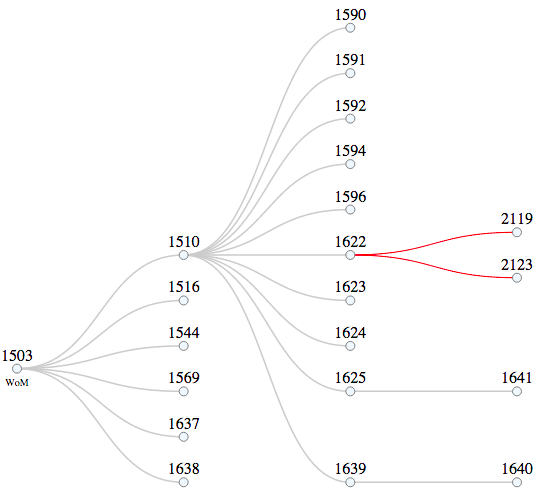
\includegraphics[width=\linewidth]{img/deep-tree.png}
	\caption{Example of Organic Spread Between Users}
	\label{fig:sustained}
\end{figure} 

\begin{figure}[t!]
	\hspace*{-2mm}
		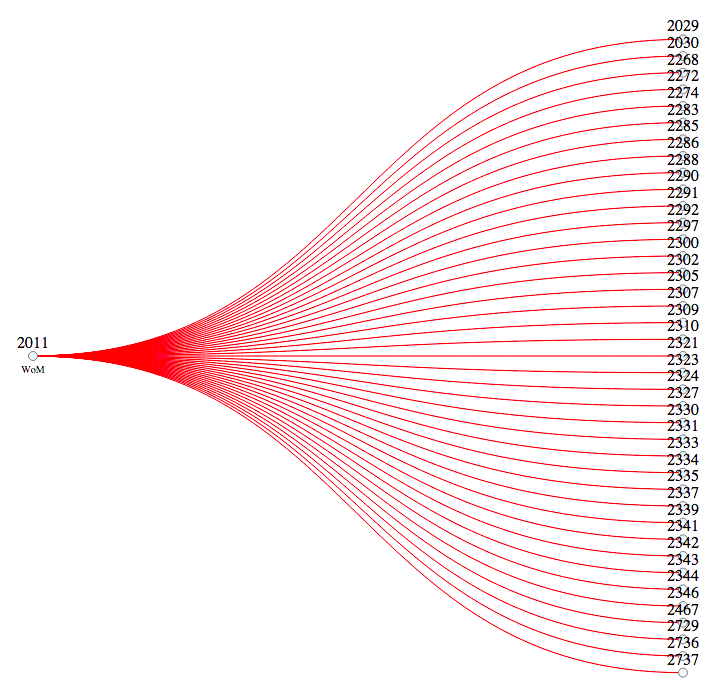
\includegraphics[width=\linewidth]{img/super-spreader.png}
	\caption{Example of Single User `Super' Spreading}
	\label{fig:super}
\end{figure}

%\section{Future Work}
Future work is fun.

\section{Conclusions}
Conclusions, etc. 
%\section{Acknowledgements}
Thank you Mr. Bigglesworth, etc. 

%\pagebreak
\eightpt
  \bibliographystyle{IEEEtran}
  
  \bibliography{bibblybib}

\end{document}
